\section{Making Payments}\label{sec:making-payments}
The sender makes payments by sending signed messages to the receiver off-chain.
Each message specifies a cumulative total amount of ether owed to the receiver, rather than the amount of the individual
micropayment.
Messages are cryptographically signed (e.g., using ECDSA) by the sender and then transmitted directly to the receiver.
This step is preformed entirely outside the Ethereum network, e.g., using email or SMS (Short Message Service).
Each message consists of two parts:

\begin{itemize}
    \item The address of the smart contract, which is used to prevent cross-contract replay attacks.
    \item The amount of ether owed to the receiver.
\end{itemize}

Payment messages can be constructed and signed in any language that supports cryptographic hashing and signing
operations.
The following example is written in Node.js JavaScript with Hardhat and ethers.js.

\verbatiminput{../scripts/SignPayment.js}

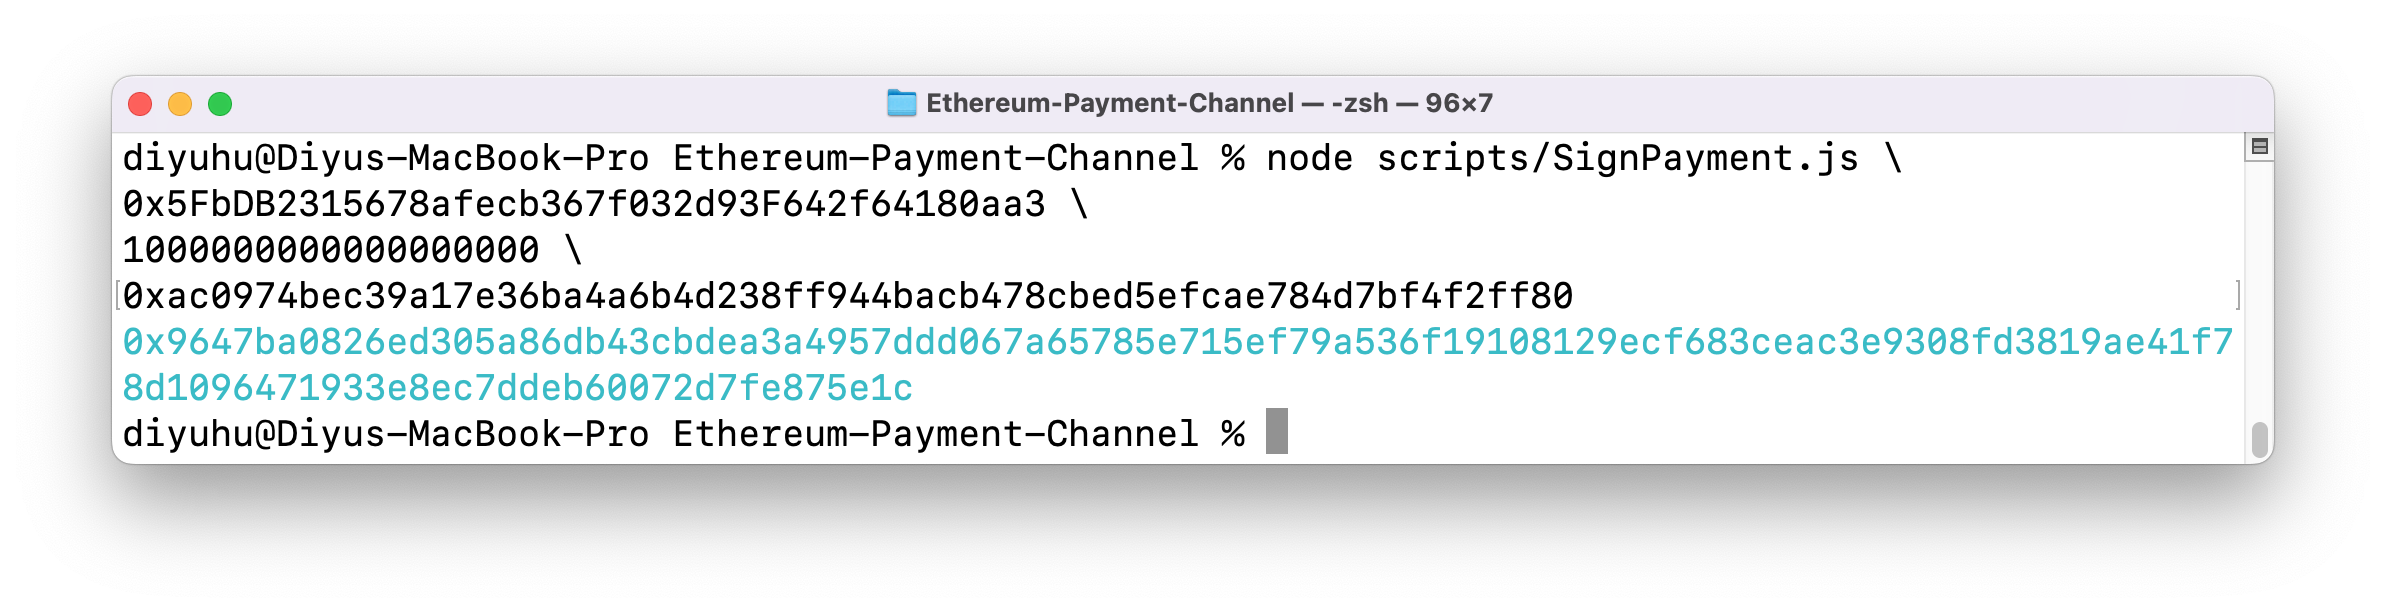
\includegraphics[width=\textwidth]{./images/sign-message-example}